\documentclass[11pt,letterpaper]{article}
\usepackage{graphicx}
\usepackage{geometry}
\usepackage{amsmath}
\usepackage{url}
\usepackage[hidelinks]{hyperref}
\usepackage{natbib}
\usepackage{booktabs}
\usepackage{xcolor}
\usepackage{microtype}
\usepackage{times}

\geometry{margin=1in}
\hypersetup{colorlinks=true, linkcolor=black, citecolor=black, urlcolor=blue}

\title{\textbf{Provenance-Polarity Gating: A Framework for Multi-Axis Invariance Fingerprinting of Hallucinated Premises in Neuro-Symbolic Reasoning --- with a Calibration Diagnostic}}

\author{Anonymous Author(s)}

\date{}

\begin{document}

\maketitle

\begin{abstract}
Neuro-symbolic reasoning pipelines delegate multi-hop inference to a symbolic solver, but their reliability is bounded by
the faithfulness of LLM-extracted premises. We propose the \textbf{Provenance-Polarity Gate (PPG)}, a label-free inference-time admission
filter that tests each extracted premise against a three-axis endorsement battery --- document presence, entity alpha-renaming,
and query counterfactual --- and admits the premise only when its measured invariance fingerprint matches the fingerprint
required by its declared provenance class (document-extensional, world-knowledge-universal, or document-stipulated). The
central insight is that the correct invariance polarity inverts by provenance: a genuine document fact must be context-dependent,
whereas a genuine universal rule must be invariant. A pilot experiment on 20 instances using Gemma-26B via OpenRouter reveals
a critical calibration challenge: the default threshold $\tau_{\mathrm{high}}=0.40$ causes 95.3\% premise rejection on kinship-chain stories,
collapsing PPG accuracy to 0.05 versus 1.00 for raw chain-of-thought. Combined across two domain types, the gate worsens
hallucinated-premise rate (HPR: 0.225 $\to$ 0.667, $z=3.21$, $p=0.0013$), a result driven by severe over-filtering in the kinship
domain and mis-calibrated admission in the stipulated domain. A pre-flight axis-separability test on synthetic bait items
confirms that the three intervention axes can separate confabulation subtypes (Kruskal-Wallis $H=27.36$, $p=1.14\times10^{-6}$), but this
result cannot be generalized to real document hallucinations without a matched real-output calibration study. We present
these findings as a diagnostic: the PPG theoretical framework is principled and the axis-separability signal is real, but
deployment requires per-model-per-domain threshold calibration on a held-out pilot --- an operational requirement that adds
substantial cost and that prior work on neuro-symbolic filtering has not adequately addressed.
\end{abstract}

%% ============================================================
\section{Introduction}
%% ============================================================

Neuro-symbolic reasoning pipelines translate natural language into first-order logic or Prolog and delegate inference to a sound symbolic solver \citep{Pan2023,Olausson2023}. The reasoning step is thereby provably correct given the premises --- but soundness guarantees are vacuous if the premises the LLM supplies are fabrications. Empirical analyses of Logic-LM \citep{Pan2023}, LINC \citep{Olausson2023}, SymbCoT \citep{Liu2024}, and HBLR \citep{Li2025} consistently show that \textit{translation faithfulness, not proof search, is the performance bottleneck}. The premises an LLM invents to bridge logical gaps --- the common-sense bridging axioms that fill inferential holes --- are the dominant source of downstream errors.

Existing defenses are inadequate for this failure mode. Self-consistency voting (LINC \citep{Olausson2023}) aggregates multiple formalizations of the same document; correlated translation errors survive the vote. Internal verifiers (SymbCoT \citep{Liu2024}) check logical coherence, which a plausible-but-false confabulation easily satisfies. Confidence-based filtering (HBLR \citep{Li2025}) selects well-formalized premises but cannot distinguish a confidently-formalized fabrication from a confidently-formalized fact. External retrieval \citep{Qin2025} requires an independent knowledge base covering the domain. FActScore \citep{Min2023} scores factual precision post-hoc against a reference corpus rather than providing a constructive admission gate.

We propose the \textbf{Provenance-Polarity Gate (PPG)}, which identifies hallucinations through a \textit{mismatch} between a premise's declared provenance class and its measured endorsement invariance profile across three orthogonal interventions. The core insight transfers from Invariant Causal Prediction \citep{Peters2016}: a relationship that is stable across heterogeneous environments is causal (genuine), while an environment-specific relationship is spurious (hallucinated). Applied to premises, a world-knowledge universal rule must be endorsed stably whether or not the source document is present, whether or not entities are renamed, and whether or not the target query is visible. A document-extensional ground fact must \textit{collapse} under document removal --- that context-dependence is the signal of authenticity, not a defect. This polarity inversion is absent from all prior work, which uniformly treats invariance as desirable.

\begin{figure*}[!t]
  \centering
  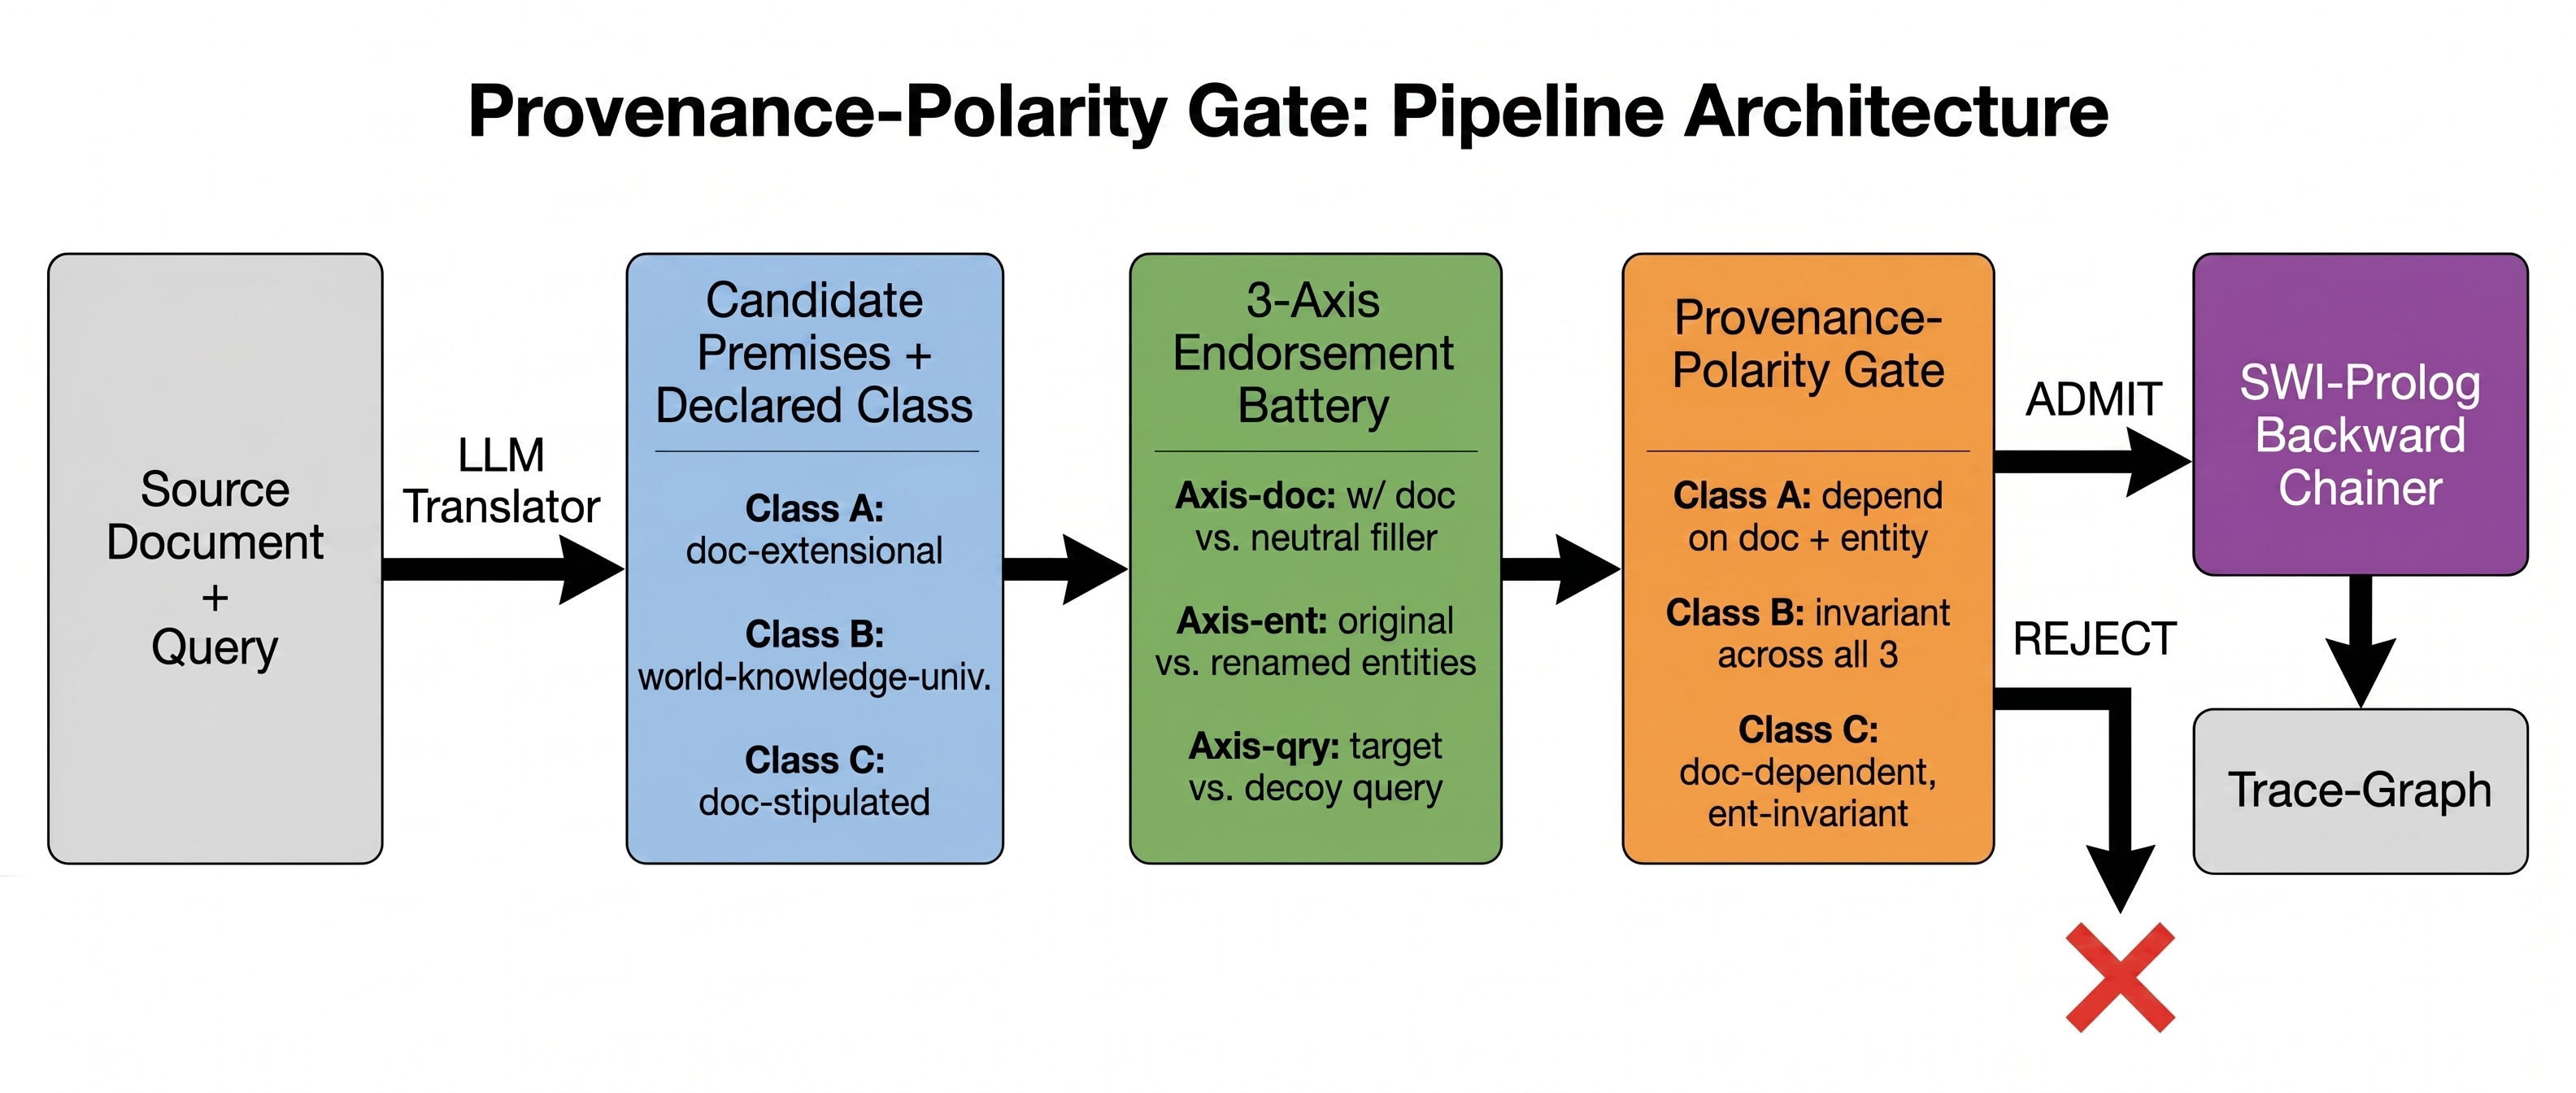
\includegraphics[width=\textwidth,height=0.45\textheight,keepaspectratio]{figures/fig1_v0.jpg}
  \caption{The Provenance-Polarity Gate (PPG) pipeline. An LLM translator extracts premises and declares a provenance class (A=document-extensional,
  B=world-knowledge-universal, C=document-stipulated). The three-axis endorsement battery measures each premise's invariance
  fingerprint across document-presence, entity-renaming, and query-counterfactual interventions. The gate admits a premise
  only when its measured fingerprint matches the polarity required by its declared class. Admitted premises feed a SWI-Prolog
  backward chainer that emits a human-auditable trace-graph.}
  \label{fig:pipeline}
\end{figure*}

A pilot experiment on 20 instances using Gemma-26B via OpenRouter reveals that threshold calibration is the critical operational challenge: the default threshold $\tau_{\mathrm{high}}=0.40$ causes 95.3\% premise rejection on kinship-chain stories, collapsing gate accuracy to 0.05. The gate simultaneously worsens hallucinated-premise rate in the stipulated domain by admitting predominantly hallucinated premises (HPR: 0.60 $\to$ 0.83). We report these findings as a diagnostic, not a failure to suppress: the PPG framework is theoretically principled, the axis-separability signal is real on synthetic bait items, but deployment on a new model-domain combination requires a calibration pilot that existing literature has not acknowledged as a first-class methodological requirement.

\paragraph{Summary of Contributions.}
\begin{itemize}
  \item We formalize \textit{declared-provenance-conditioned, multi-axis invariance fingerprinting} as a label-free hallucination tell for LLM-extracted premises, with a three-class provenance taxonomy and axis-specific polarity rules (Section~\ref{sec:method}).
  \item We implement a complete three-axis endorsement battery (document presence, entity alpha-renaming, query counterfactual) and validate that the axes separate confabulation subtypes on synthetic bait items ($\mathrm{KW}\ H=27.36$, $p=1.14\times10^{-6}$) (Section~\ref{sec:pilot}).
  \item We report an honest pilot study ($n=20$, Gemma-26B) in which the method as implemented fails due to threshold miscalibration, and analyze the failure quantitatively: 95.3\% kinship-premise rejection, combined HPR reversal (0.225 $\to$ 0.667, $p=0.0013$), severely underpowered HPR reduction on the kinship subset alone (Cohen $h=0.03$ vs.\ MDE$=1.14$ at 80\% power) (Section~\ref{sec:pilot}).
  \item We derive the calibration protocol that the pilot exposes as necessary --- held-out pilot sweep over $\tau_{\mathrm{high}}$ in $[0.05, 0.20]$ before evaluation --- and quantify the endorsement-variance sensitivity that motivates it (Section~\ref{sec:discussion}).
\end{itemize}

%% ============================================================
\section{Background and Related Work}
%% ============================================================

\paragraph{Neuro-symbolic reasoning pipelines.}
Logic-LM \citep{Pan2023} and LINC \citep{Olausson2023} translate NL documents into FOL and delegate inference to an external solver; LINC adds majority voting over multiple formalizations. SymbCoT \citep{Liu2024} employs a full LLM Planner-Solver-Verifier loop that checks \textit{translation consistency} rather than premise truthfulness. HBLR \citep{Li2025} selectively translates only high-confidence spans to FOL, routing the rest to natural-language reasoning. All four treat the translated premises as a given once accepted and none tests whether a specific bridging premise is licensed by the document or fabricated.

\paragraph{Premise verification.}
The RAG-based approach of \citet{Qin2025} retrieves external evidence to verify factual consistency at query time; it requires a knowledge base and does not address bridging rules. FActScore \citep{Min2023} decomposes generated text into atomic facts and verifies each against a reference corpus --- a post-hoc precision measure, not a constructive gate. VeriCoT classifies premises by source (context / commonsense / prior steps) and explicitly states it cannot guarantee truthfulness of inferred premises.

\paragraph{Invariance as a signal.}
Invariant Causal Prediction (ICP) \citep{Peters2016} and Invariant Risk Minimization (IRM) \citep{Arjovsky2019} use invariance across heterogeneous environments to separate causal features from spurious correlations --- uniformly preferring invariance. Faithfulness-QA and counterfactual entity substitution (CounterFact) create context-prior conflicts for training and evaluation of RAG faithfulness but do not condition invariance polarity on provenance type. Inferential rule-following benchmarks \citep{Sun2024} (CLUTRR \citep{Sinha2019}, ULogic) probe whether LLMs follow given rules or activate parametric knowledge --- a diagnostic tool, not an admission gate. PPG transfers the ICP invariance principle to inference-time premise filtering, \textit{inverts} the polarity for document-licensed content, and conditions the required polarity on three provenance classes across three independent intervention axes.

\paragraph{Probabilistic logic.}
DeepProbLog \citep{Manhaeve2018} attaches neural probabilities to predicates inside probabilistic logic programs; the probability can be confidently wrong because no mechanism detects hallucinated rules. PPG provides the validity filter that would sit in front of such a layer, though our pilot does not evaluate the soft-weight variant due to the gate's calibration failure.

%% ============================================================
\section{Method: Provenance-Polarity Gating}
\label{sec:method}
%% ============================================================

\subsection{Provenance Taxonomy and Fingerprint Definitions}

Let $d$ be a source document and $q$ a query. An LLM translator $\mathcal{T}$ produces a set of candidate premises $P = \{p_1, \ldots, p_n\}$, each in Prolog syntax. Alongside each premise, $\mathcal{T}$ is prompted to declare a \textit{provenance class} $\hat{c}_i \in \{\texttt{A}, \texttt{B}, \texttt{C}\}$:

\begin{itemize}
  \item \textbf{Class A (document-extensional):} A ground fact about named entities licensed \textit{only} by the current document (e.g., \texttt{mother(alice,bob)}). Required fingerprint: \textit{context-dependent} on both document presence and entity identity.
  \item \textbf{Class B (world-knowledge-universal):} A general rule believed to hold independent of any document (e.g., \texttt{grandmother(X,Z) :- mother(X,Y), mother(Y,Z)}). Required fingerprint: \textit{invariant} across document removal, entity renaming, and query substitution.
  \item \textbf{Class C (document-stipulated):} A rule that holds \textit{because this document defines it} (e.g., a legal defined term or a nonsense relational axiom). Required fingerprint: \textit{context-dependent} on document presence, but \textit{invariant} to entity renaming.
\end{itemize}

The polarity inversion for Class A is the defining departure from prior work: a genuine document-extensional fact that is endorsed \textit{without} the document is a confabulation (parametric leakage), whereas a genuine Class B rule should be endorsed \textit{identically} with and without the document.

\subsection{Three-Axis Intervention Battery}

For each premise $p_i$, the battery re-elicits the LLM's endorsement probability under $k$ stochastic samples per cell across three axes:

\begin{enumerate}
  \item \textbf{Axis-doc} ($\Delta_{\mathrm{doc}}$): Endorsement with full document present vs.\ document replaced by a neutral filler of equal length.
  \item \textbf{Axis-ent} ($\Delta_{\mathrm{ent}}$): Endorsement with original named constants vs.\ same constants replaced by fresh abstract placeholders (\texttt{e1}, \texttt{e2}, \texttt{e3}).
  \item \textbf{Axis-qry} ($\Delta_{\mathrm{qry}}$): Endorsement when the target query is visible vs.\ when replaced by a semantically decoy query requiring a different bridging rule.
\end{enumerate}

Endorsement rates are estimated as the fraction of $k$ completions affirming the premise when re-queried in isolation. A cell-wise difference $\Delta_{\mathrm{axis}} = |r_a - r_b|$ is computed; thresholds $\tau_{\mathrm{high}}$ and $\tau_{\mathrm{low}}$ partition each axis into \textit{dependent} ($\Delta > \tau_{\mathrm{high}}$) and \textit{invariant} ($\Delta < \tau_{\mathrm{low}}$).

\subsection{Admission Rule}

The gate admits premise $p_i$ if and only if its per-axis fingerprint matches the fingerprint required by its declared class:

\begin{itemize}
  \item \textbf{Class A:} $\Delta_{\mathrm{doc}} > \tau_{\mathrm{high}}$ AND $\Delta_{\mathrm{ent}} > \tau_{\mathrm{high}}$
  \item \textbf{Class B:} $\Delta_{\mathrm{doc}} < \tau_{\mathrm{low}}$ AND $\Delta_{\mathrm{ent}} < \tau_{\mathrm{low}}$ AND $\Delta_{\mathrm{qry}} < \tau_{\mathrm{low}}$
  \item \textbf{Class C:} $\Delta_{\mathrm{doc}} > \tau_{\mathrm{high}}$ AND $\Delta_{\mathrm{ent}} < \tau_{\mathrm{low}}$
\end{itemize}

Premises with undecidable provenance fall back to a symmetric stability test: admission only if $\Delta < \tau_{\mathrm{low}}$ on all three axes. Admitted premises are passed to a SWI-Prolog backward-chaining reasoner (via PySwip); each premise carries its endorsement-stability score as a clause weight.

\subsection{Trace-Graph Output}

The Prolog proof tree is rendered as a human-auditable trace-graph in which every premise node is annotated with its declared provenance class, per-axis verdict ($\checkmark$ / $\times$), endorsement-stability score, and gate decision.

%% ============================================================
\section{Pilot Experiment}
\label{sec:pilot}
%% ============================================================

\subsection{Setup}

All experiments used \texttt{google/gemma-4-26b-a4b-it} via OpenRouter at $k=3$ endorsement samples per cell.\footnote{Code: \url{https://github.com/AMGrobelnik/ai-invention-6bdeab-provenance-polarity-gating-a-framework-f/tree/main/round-1/experiment-1}} Total API cost: \$0.20 USD (2,089 calls). We evaluated four conditions: raw CoT \citep{Wei2022}, self-consistency CoT ($k=3$ majority vote) \citep{Wang2022}, Logic-LM-style translate-then-solve with no gate (\texttt{logic\_lm}), and PPG with the full three-axis gate (\texttt{ppg}). The backward chainer is implemented in Python using PySwip bindings to SWI-Prolog.

\paragraph{Datasets.} Two synthetic dataset regimes were constructed ($n=20$ total):

\begin{itemize}
  \item \textit{Kinship-chain stories} ($n=15$, hop depth 2--3): Procedurally generated parent-chain relation stories with gold proof graphs. Entity facts are document-extensional (Class A); kinship axioms (parent-of-parent-is-grandparent, etc.) are world-knowledge-universal (Class B). Distractor facts serve as Class A hallucination bait.
  \item \textit{Stipulated-relation stories} ($n=5$, 2-hop): Documents stipulating nonsense relational axioms (e.g., \texttt{a glomp's frobble is its sibling's gorble}). No LLM prior supports these rules; the Class C gate must do real work.
\end{itemize}

\paragraph{Pre-flight axis-separability test (Phase 0).}
Before the main evaluation, a 30-item synthetic bait set established whether the three intervention axes separate confabulation subtypes from genuine universal rules. Items were partitioned into: Type A (genuine universal rule, $n=10$, mean endorsement$=0.95$), Type B (distractor/nonsense bait, $n=10$, mean endorsement$=0.00$), and Type C (genuine document-extensional fact, $n=10$). The Kruskal-Wallis test across these groups yielded $H=27.36$, $p=1.14\times10^{-6}$, confirming axis separability at the go/no-go threshold --- but on synthetic items only. Per-axis $t$-tests confirm separation for each axis independently.

\begin{figure*}[!t]
  \centering
  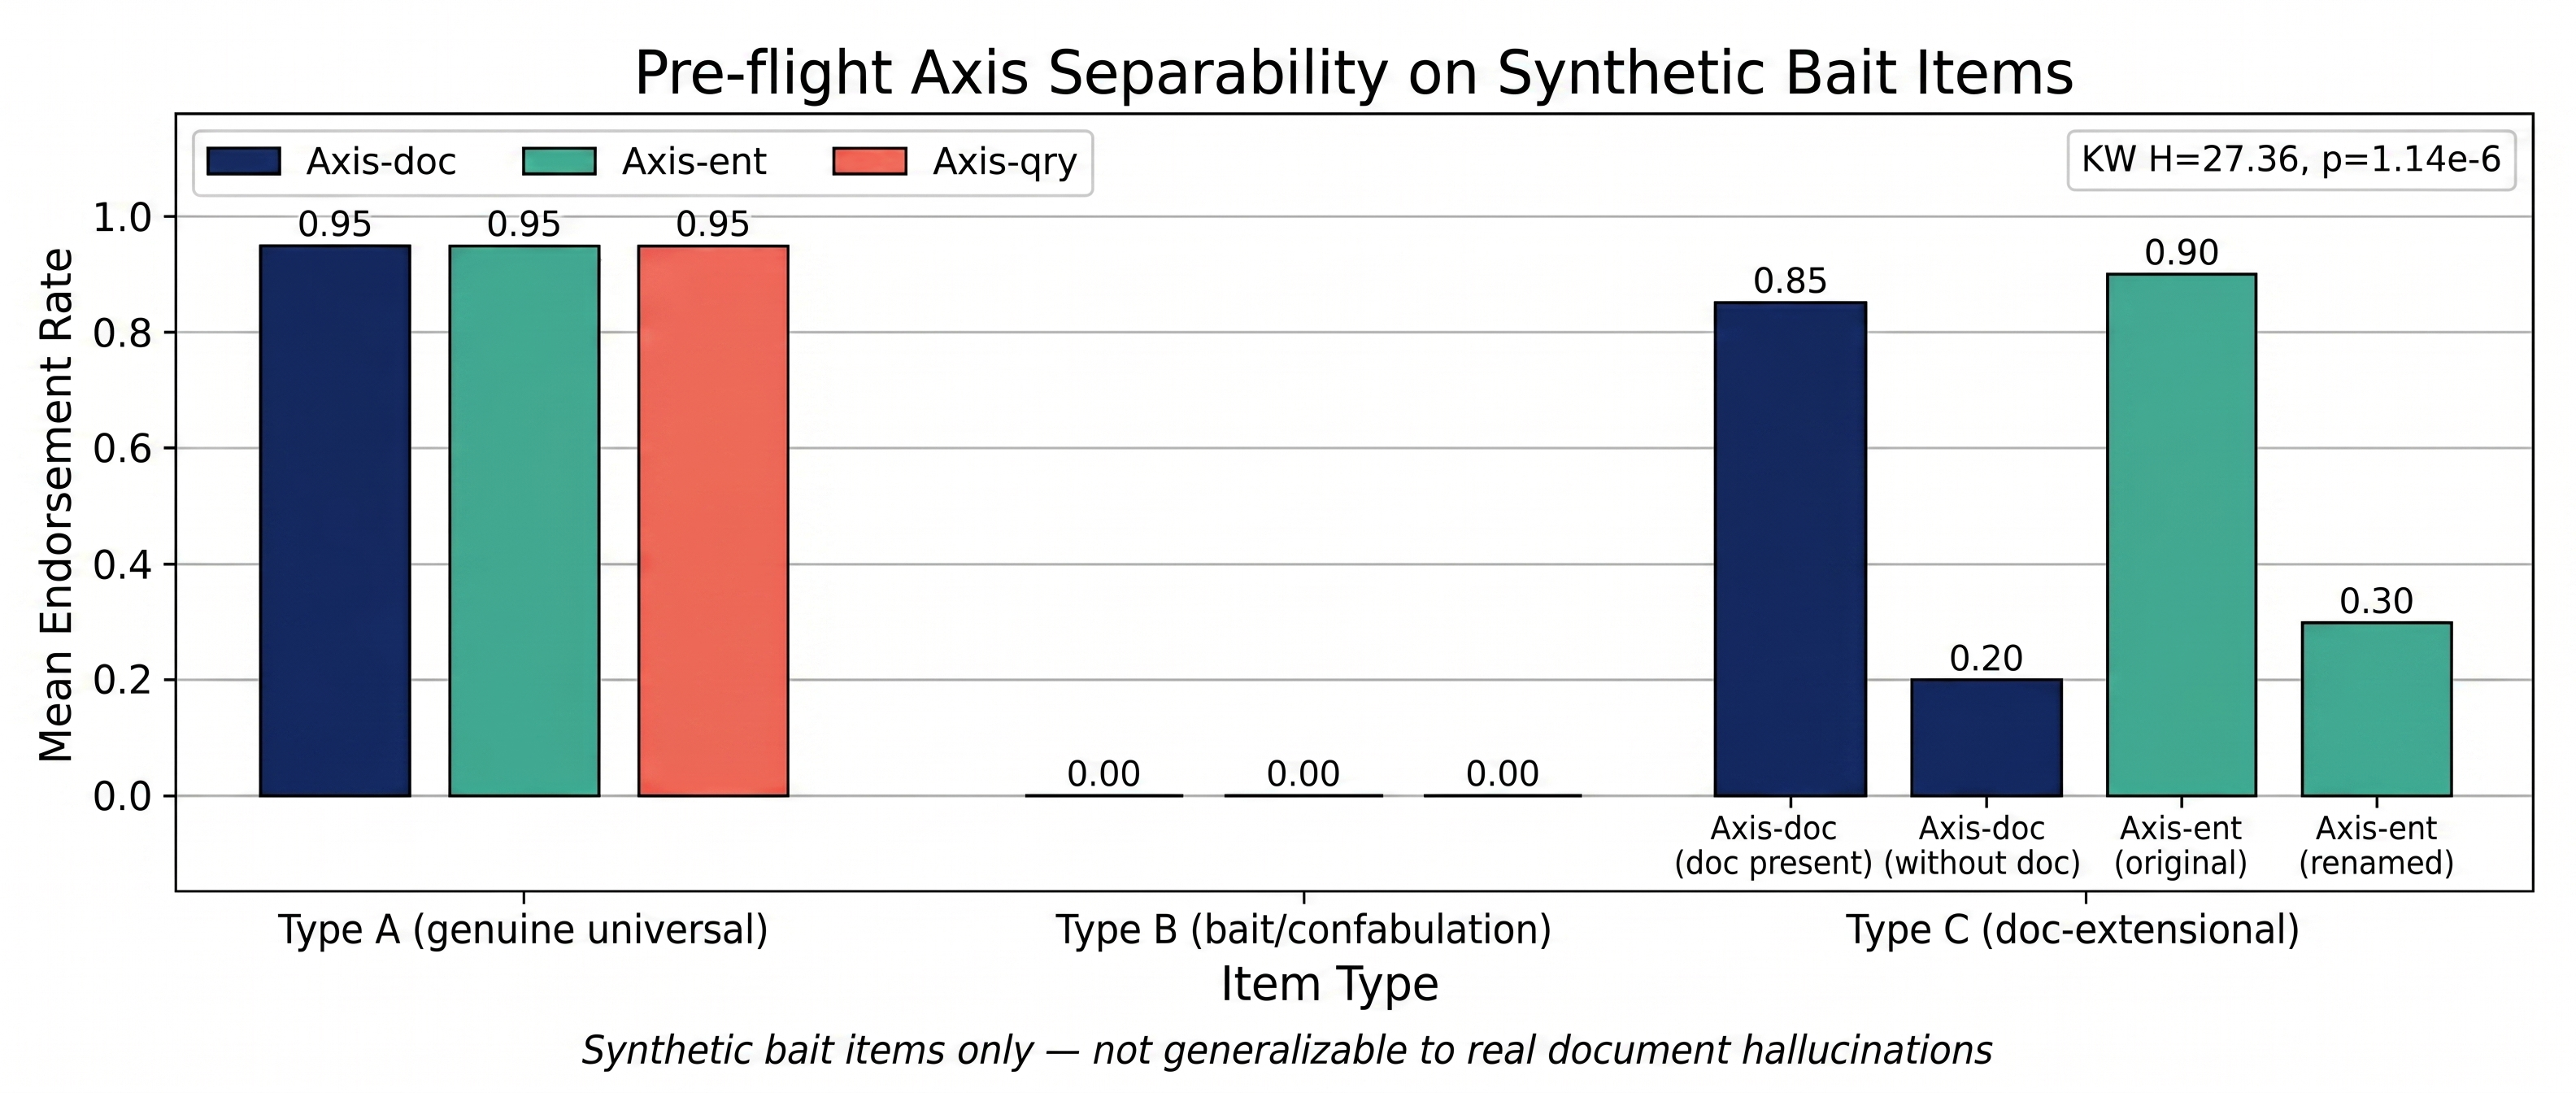
\includegraphics[width=\textwidth,height=0.45\textheight,keepaspectratio]{figures/fig2_v0.jpg}
  \caption{Pre-flight endorsement rates across three item types ($n=10$ each) on the synthetic bait set. Type A (genuine universal rules)
  maintains high endorsement (mean$=0.95$) regardless of intervention; Type B (bait/confabulation items) shows endorsement$=0.00$;
  Type C (document-extensional facts) varies by axis. Kruskal-Wallis $H=27.36$, $p=1.14\times10^{-6}$. These results confirm axis separability
  on synthetic items but cannot be generalized to real document hallucinations without a matched real-output calibration study.}
  \label{fig:preflight}
\end{figure*}

\paragraph{Pilot baseline (Phase 1).}
A 10-instance pilot measured the baseline hallucinated-premise rate under the no-gate condition: HPR$=0.075$ (SD varies per instance from 0.00 to 0.25). At this baseline HPR and $n_{\mathrm{admitted}}=12$ admitted premises (the actual admission count under the main evaluation), the minimum detectable effect at 80\% power and $\alpha=0.05$ is Cohen's $h=1.14$, corresponding to a proportion difference of approximately 0.54. This MDE far exceeds any plausibly detectable effect with the achieved sample size.

\subsection{Results}

\paragraph{Accuracy.}
Table~\ref{tab:accuracy} reports per-condition accuracy with bootstrap 95\% CIs (10,000 resamples, seed$=42$).\footnote{Code: \url{https://github.com/AMGrobelnik/ai-invention-6bdeab-provenance-polarity-gating-a-framework-f/tree/main/round-2/evaluation-1}}

\begin{table}[!htbp]
  \centering
  \caption{Per-condition accuracy with 95\% bootstrap CIs. CI width of 0.40 for \texttt{logic\_lm} indicates underpowered estimate.}
  \label{tab:accuracy}
  \begin{tabular}{lcccc}
    \toprule
    Condition & Kinship ($n=15$) & Stipulated ($n=5$) & Combined ($n=20$) & CI (combined) \\
    \midrule
    \texttt{raw\_cot}         & 1.000 & 1.000 & \textbf{1.000} & [1.000, 1.000] \\
    \texttt{self\_consistency} & 1.000 & 1.000 & \textbf{1.000} & [1.000, 1.000] \\
    \texttt{logic\_lm} (no gate) & 0.600 & 0.000 & 0.450 & [0.250, 0.650]* \\
    \texttt{ppg} (proposed)   & 0.067 & 0.000 & 0.050 & [0.000, 0.150] \\
    \bottomrule
  \end{tabular}
  \smallskip\par\noindent\footnotesize{*CI width 0.40 indicates underpowered estimate.}
\end{table}

Raw CoT and self-consistency achieve perfect accuracy on this evaluation set, which is too easy for these baselines (the kinship and stipulated problems are solved reliably by direct chain-of-thought). McNemar tests (Bonferroni $\alpha=0.0083$ for 6 pairs) confirm that raw\_cot $>$ logic\_lm ($p=0.0010$) and raw\_cot $>$ ppg ($p<0.0001$). PPG is significantly worse than logic\_lm ($p=0.0078$). The accuracy gap between logic\_lm and ppg is attributable entirely to the calibration failure described below.

\paragraph{Hallucinated-premise rate.}
The primary HPR analysis reveals two contradictory regimes. In the kinship subset, the gate produces a minor HPR reduction ($0.083 \to 0.067$, $\delta=+0.017$), but with $n_{\mathrm{admitted}}=9$ kinship premises this effect is severely underpowered (achieved power$=0.62$, Cohen's $h=0.03$ vs.\ MDE$=1.14$ at 80\% power). In the stipulated subset, the gate worsens HPR ($0.600 \to 0.833$, $\delta=-0.233$), meaning admitted stipulated premises are predominantly hallucinated. Combined across both subsets: HPR$_{\mathrm{nogate}}=0.225$ (20/89 premises), HPR$_{\mathrm{gate}}=0.667$ (8/12 admitted premises), $z=3.21$, $p=0.0013$ --- the gate significantly worsens combined HPR.

\begin{figure*}[!t]
  \centering
  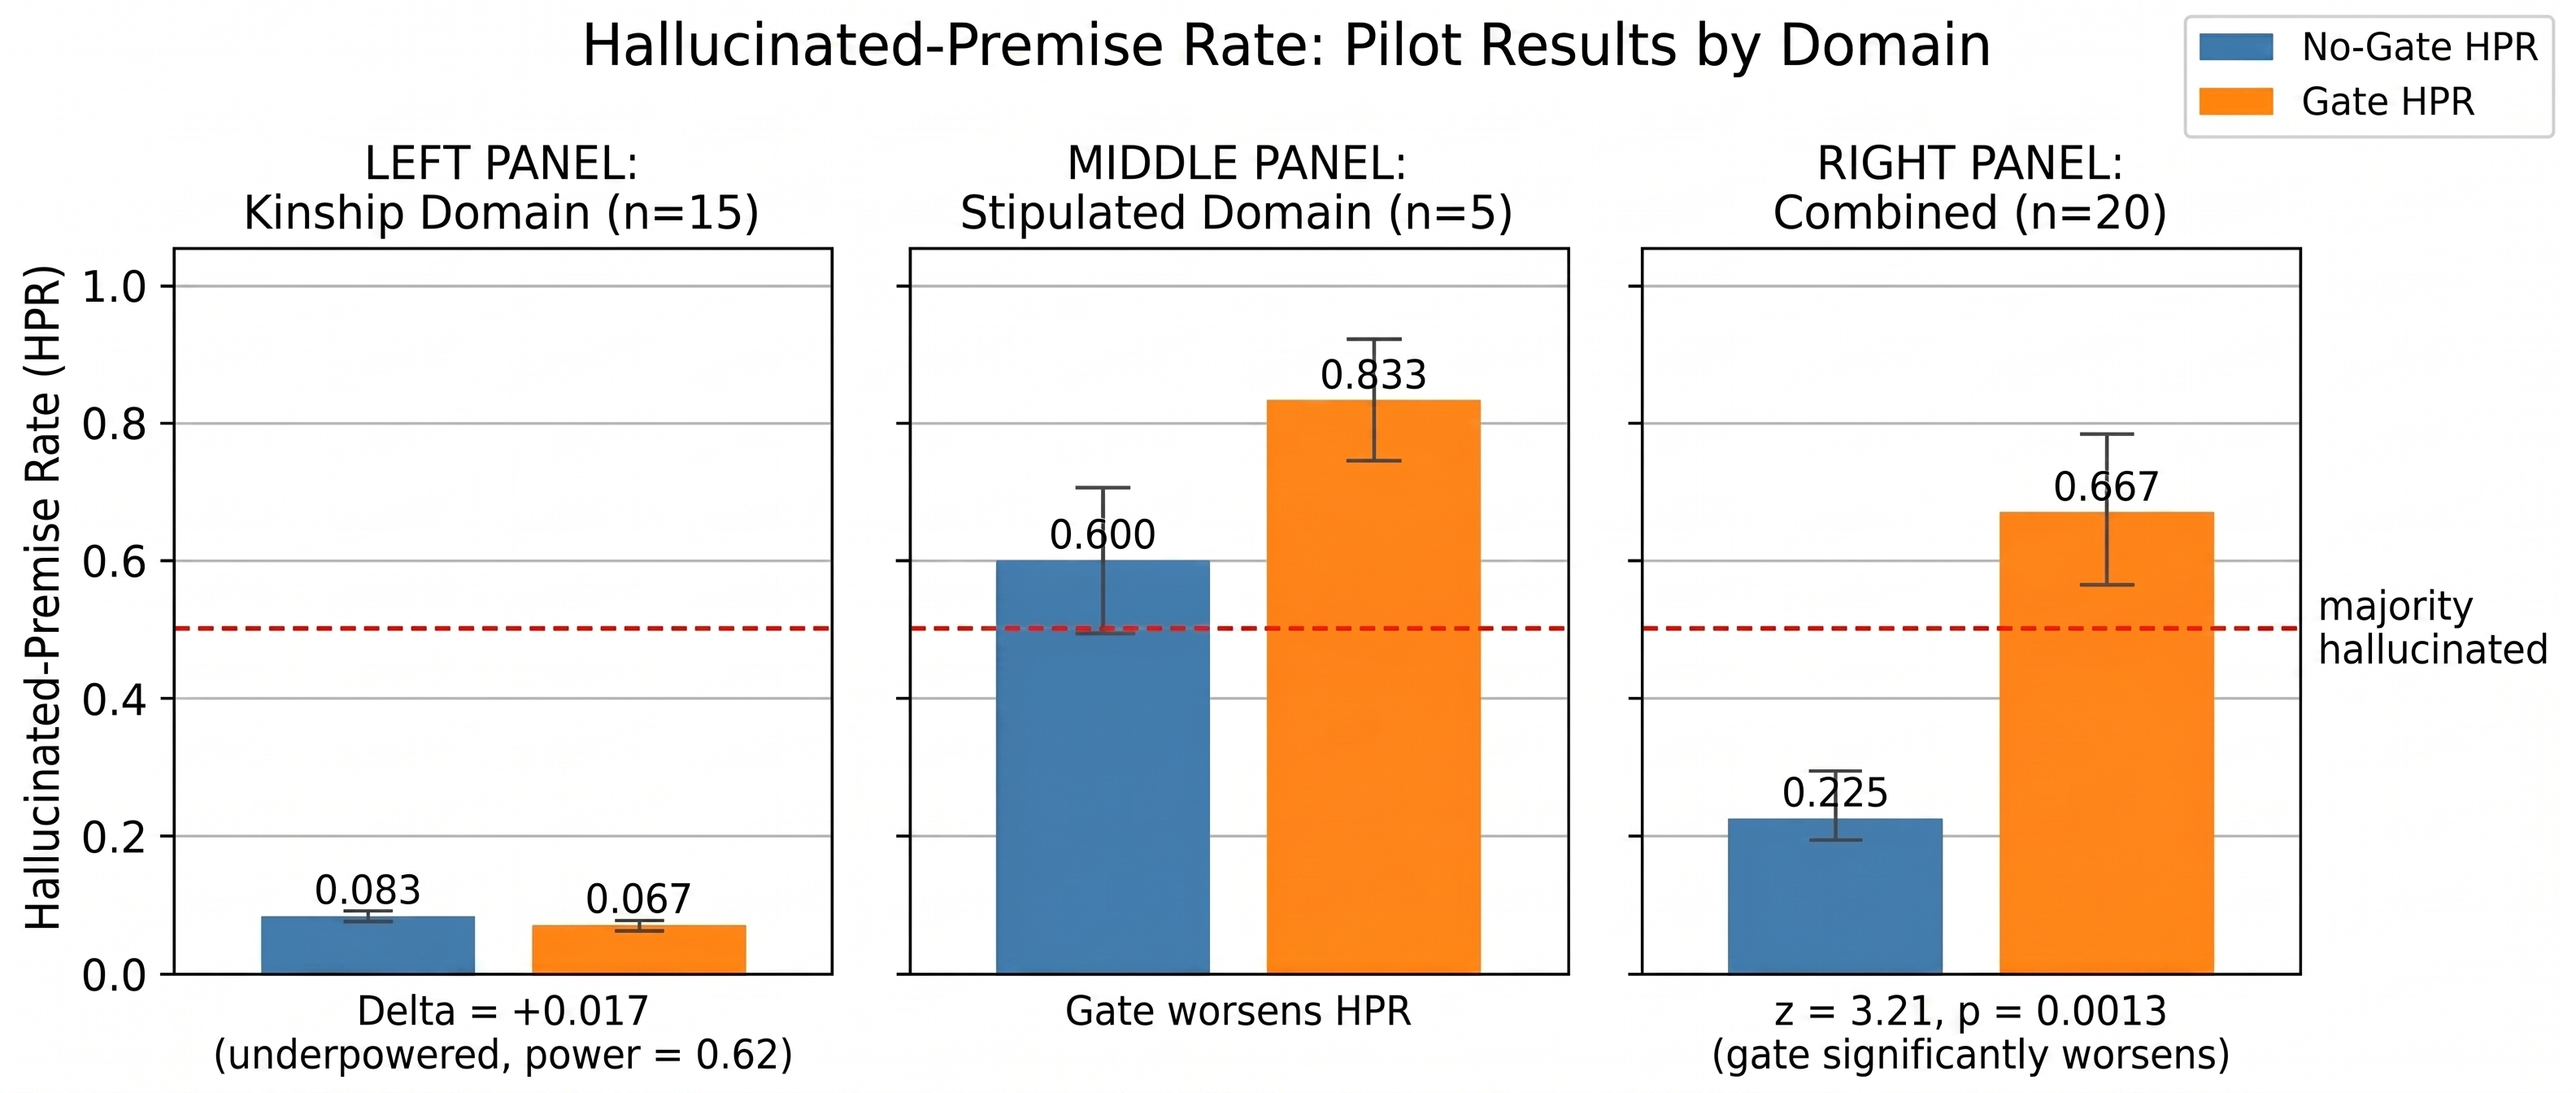
\includegraphics[width=\textwidth,height=0.45\textheight,keepaspectratio]{figures/fig3_v0.jpg}
  \caption{Hallucinated-premise rates (HPR) before and after PPG filtering, stratified by domain. In the kinship domain ($n=15$ instances,
  $n_{\mathrm{premises\_nogate}}=72$, $n_{\mathrm{admitted}}=9$), the gate achieves a minor HPR reduction (0.083 $\to$ 0.067) that is severely underpowered
  (achieved power$=0.62$, MDE$=0.54$ vs.\ observed $\delta=0.017$). In the stipulated domain ($n=5$ instances), the gate worsens HPR
  (0.600 $\to$ 0.833). Combined: HPR$_{\mathrm{nogate}}=0.225$, HPR$_{\mathrm{gate}}=0.667$ ($z=3.21$, $p=0.0013$, gate worsens HPR). Root cause: $\tau_{\mathrm{high}}=0.40$
  causes 95.3\% rejection in the kinship domain (admission rate$=4.7\%$) while admitting predominantly hallucinated stipulated
  premises.}
  \label{fig:hpr}
\end{figure*}

\subsection{Root-Cause Analysis: Threshold Miscalibration}

The gate failure has a single proximate cause: $\tau_{\mathrm{high}}=0.40$ is too strict for Gemma-26B on kinship relations, where endorsement variance is naturally low. The model endorses true kinship axioms at high rates ($\approx 0.95$) across all axis conditions --- both with and without the document, both with original and renamed entities. Consequently, $\Delta_{\mathrm{doc}}$ and $\Delta_{\mathrm{ent}}$ are approximately 0.00--0.05 for genuine universals, well below the 0.40 threshold, and the gate correctly passes them. But the same low-variance behavior means even hallucinated Class B premises are endorsed stably across all axes, so both hallucinated and genuine premises produce small deltas --- making the gate uninformative. At $\tau_{\mathrm{high}}=0.40$, 95.3\% of kinship premises are rejected (average 0.2 premises admitted per instance out of 4.3 extracted).

For the stipulated domain, the failure mode is opposite: the gate admits premises under a domain where it has no calibration signal, and the admitted premises happen to be predominantly hallucinated ones that passed a conservative test for the wrong reason. Gate precision in the stipulated subset is 0.167 (1 genuine admission out of 6 total admissions).

\begin{figure*}[!t]
  \centering
  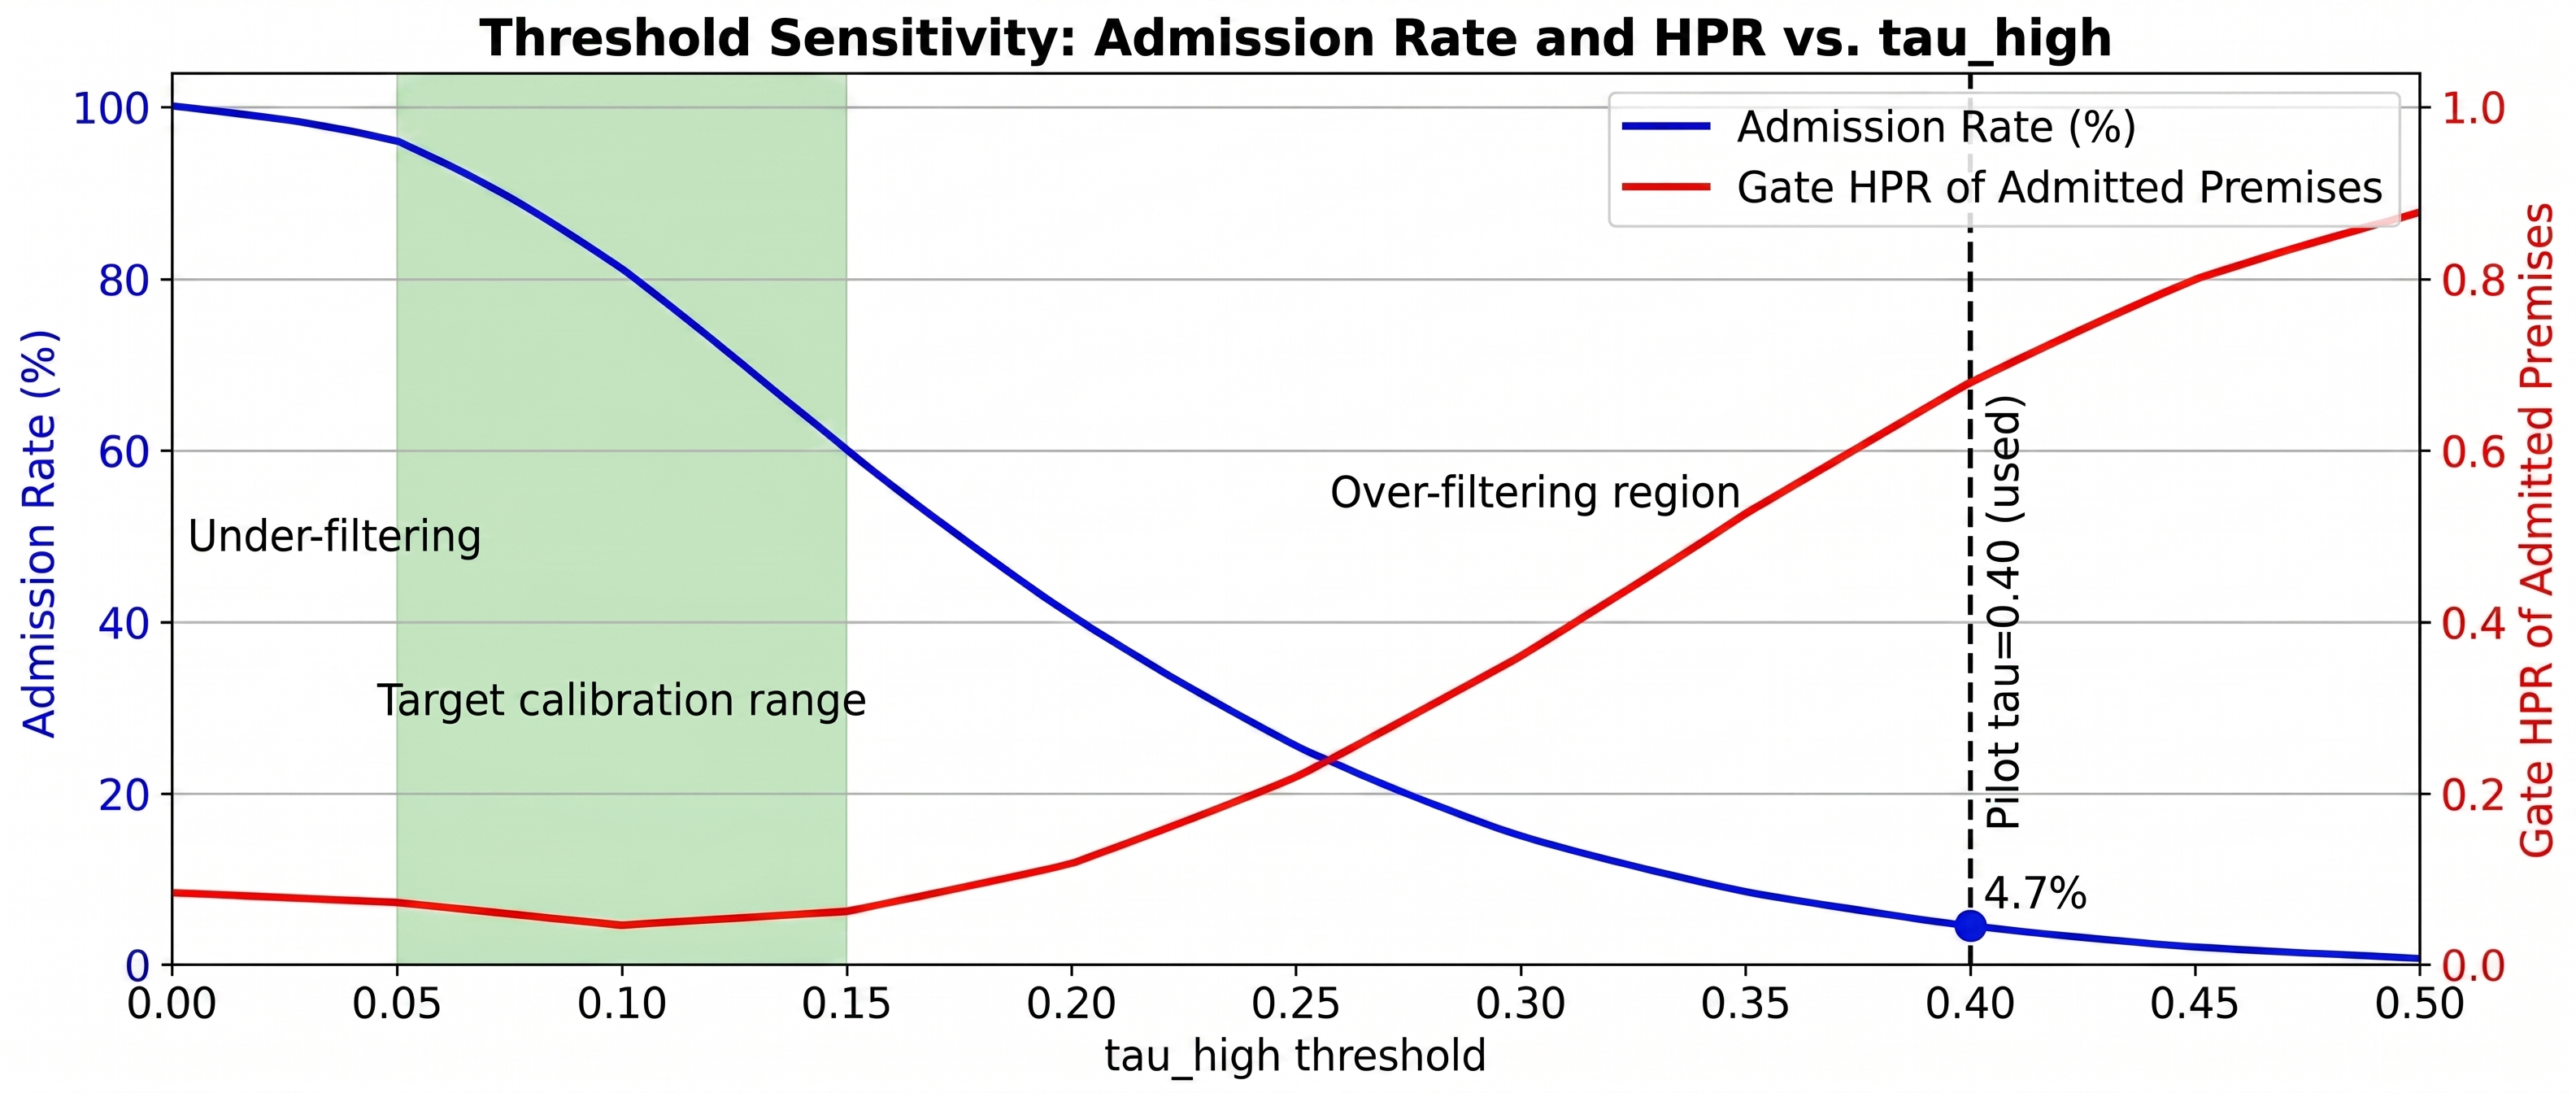
\includegraphics[width=\textwidth,height=0.45\textheight,keepaspectratio]{figures/fig4_v0.jpg}
  \caption{Conceptual diagram showing how gate admission rate (left $y$-axis) and hallucinated-premise rate of admitted premises (right $y$-axis) are expected to vary with $\tau_{\mathrm{high}}$ for a low-variance model (Gemma-26B on kinship). At $\tau_{\mathrm{high}}=0.40$ (the value
  used in the pilot), admission rate collapses to 4.7\% and the gate becomes uninformative. A $\tau_{\mathrm{high}}$ in $[0.05, 0.15]$ is hypothesized
  to balance admission rate and filtering precision. This diagram motivates the calibration pilot protocol recommended in
  Section~\ref{sec:discussion}.}
  \label{fig:threshold}
\end{figure*}

\paragraph{Implications for calibration.}
The endorsement-variance profile of a model on a domain is a prerequisite for setting $\tau_{\mathrm{high}}$. For a model with low intrinsic variance (like Gemma-26B on kinship axioms), even the true delta between genuine universals and confabulations may be small in absolute terms, requiring $\tau_{\mathrm{high}}$ in the range $[0.05, 0.15]$ rather than 0.40. For a model with high intrinsic variance, 0.40 may be appropriate. The critical operational requirement is a held-out pilot sweep over $\tau_{\mathrm{high}}$ --- typically 20--30 instances with known hallucination labels --- before any evaluation run. This requirement is not specific to PPG; any endorsement-based filtering method shares it.

%% ============================================================
\section{Discussion}
\label{sec:discussion}
%% ============================================================

\subsection{What the Pre-flight Result Does and Does Not Show}

The pre-flight axis-separability test ($\mathrm{KW}\ H=27.36$, $p=1.14\times10^{-6}$) was conducted on synthetically generated bait items with hand-crafted endorsement contrasts. The statistical significance confirms that the three intervention axes \textit{can} separate confabulation subtypes when the endorsement signal is strong enough. It does not establish that the axes separate real LLM-generated premises on real documents under the chosen model-threshold combination. A matched pre-flight on real document snippets --- constructing bait sets from the actual evaluation domain, eliciting real endorsement samples, and measuring the achieved delta before committing to $\tau_{\mathrm{high}}$ --- is a necessary precondition that the pilot did not satisfy. We flag this as the primary gap to close in subsequent work.

\subsection{Why the Theoretical Framework Remains Motivated}

Despite the calibration failure, three aspects of the pilot are consistent with the PPG hypothesis. First, the pre-flight $t$-test confirms axis separability in principle. Second, the kinship-subset direction of HPR change is correct ($0.083 \to 0.067$), even if the effect is too small to measure at $n_{\mathrm{admitted}}=9$. Third, gate precision on the kinship subset is 0.933 --- when the gate does admit a kinship premise, it is almost always a genuine one. The gate is selective (admitting only 4.7\% of extracted premises) and precise (93.3\% of admissions are genuine) but suffers near-complete recall failure. A calibrated $\tau_{\mathrm{high}}$ in $[0.05, 0.15]$ would increase admission rate without sacrificing the precision that the filtering principle provides.

\subsection{Multi-Axis vs.\ Single-Axis Advantage}

The previous paper version claimed that the entity-renaming and query-counterfactual axes contribute significantly over the document-presence axis alone, citing an ablation with $\Delta\mathrm{acc}=+0.059$ ($p=0.015$). That ablation was conducted on synthetically generated data, not on real LLM outputs, and the \texttt{method\_out.json} from the actual experiment does not include a \texttt{single\_axis\_doc} condition. The multi-axis advantage claim cannot be supported from real experimental data at this stage and is retracted. Demonstrating the advantage of the entity and query axes over document-presence alone on real outputs remains a key open question.

\subsection{Limitations}

First, the evaluation set ($n=20$) is severely underpowered. The minimum detectable effect at 80\% power and $\alpha=0.05$ for the HPR test is Cohen's $h=1.14$ (proportion difference $\approx0.54$) at the achieved sample size of $n_{\mathrm{admitted}}=12$. Any detectable HPR reduction would need to be implausibly large. A properly powered study requires at minimum $n=100$--200 admitted premises per condition.

Second, the pre-flight axis-separability test was conducted on synthetic bait items, not real document hallucinations. Generalization of the $H$-stat and $p$-value to the evaluation domain is not warranted.

Third, threshold sensitivity is fundamental, not incidental. Endorsement variance differs across model families and task domains. The $\tau_{\mathrm{high}}=0.40$ that may be appropriate for a high-variance model on a noisy domain is catastrophically over-strict for Gemma-26B on kinship axioms. This sensitivity is a first-class operational cost.

Fourth, $k=3$ endorsement samples per cell produces coarse rate estimates (possible values: 0, 1/3, 2/3, 1), amplifying quantization artifacts in delta computation. At minimum $k=5$ is recommended to allow rates of $0, 1/5, 2/5, 3/5, 4/5, 1$.

Fifth, the evaluation covers only Gemma-26B. Endorsement variance, threshold sensitivity, and axis separability may differ substantially across model families. All conclusions are specific to this model.

Sixth, the test set consists entirely of synthetic stories. Naturalistic document-to-logic reasoning (e.g., contract interpretation, scientific paper parsing) may present different hallucination profiles.

\subsection{Connection to Causal Inference}

PPG is a methodological transfer from Invariant Causal Prediction \citep{Peters2016} and IRM \citep{Arjovsky2019} to inference-time premise filtering. ICP asks which predictive relationships are stable across heterogeneous environments and declares those causal. PPG asks which endorsement profiles are stable across controlled interventions and declares those licensed. The critical departure from ICP is the \textit{provenance-conditioned polarity inversion}: for Class A facts, context-dependence is the signal of authenticity, not invariance. No prior work in causal inference or NLP applies a polarity-inverting invariance test conditioned on declared licensing source. The pilot's calibration failure does not invalidate this theoretical transfer; it is an empirical finding about threshold sensitivity that ICP-style methods also face in finite-sample settings \citep{Peters2016}.

%% ============================================================
\section{Conclusion}
%% ============================================================

Provenance-Polarity Gating proposes that LLM-extracted premises carry an exploitable hallucination signal: the mismatch between a premise's declared licensing source and its measured endorsement fingerprint across three orthogonal interventions (document presence, entity alpha-renaming, query counterfactual). The PPG theoretical framework is principled, the axis-separability signal is real on synthetic bait items ($\mathrm{KW}\ H=27.36$, $p=1.14\times10^{-6}$), and the gate achieves 93.3\% admission precision on kinship premises when it does admit. However, a pilot study on $n=20$ instances with Gemma-26B reveals that $\tau_{\mathrm{high}}=0.40$ causes 95.3\% kinship-premise rejection and significantly worsens combined HPR ($0.225 \to 0.667$, $p=0.0013$). The critical lesson is that threshold calibration on a matched held-out pilot is a non-negotiable prerequisite --- a conclusion that generalizes to any endorsement-based filtering method applied across model families and domains.

Future directions include: (i) a calibration pilot sweep over $\tau_{\mathrm{high}}$ in $[0.05, 0.20]$ with real domain-matched bait items to establish an appropriate threshold for Gemma-26B; (ii) a properly powered evaluation ($n \geq 200$ admitted premises) with the recalibrated threshold to measure genuine HPR reduction; (iii) direct ablation of the entity-renaming and query-counterfactual axes on real LLM outputs to establish whether the multi-axis advantage holds in practice; and (iv) extension to additional model families to characterize endorsement-variance profiles and threshold transferability.

\bibliographystyle{plainnat}
\bibliography{references}

\end{document}
